\documentclass[14pt]{memoir}

\usepackage[paperwidth=19.0in, paperheight=13.0in]{geometry}

\newcommand{\length}[2]{\newlength#1\setlength#1{#2}}
\length\bookheight{9.61in}
\length\bookwidth{6.69in}
\length\spinewidth{0.64in}
\length\bleedmargin{0.125in}

\usepackage{tikz}

\tikzstyle{book page}=[
    minimum height=\bookheight,
    minimum width=\bookwidth
]
\tikzstyle{spine}=[
    minimum width=\bookheight,
    minimum height=\spinewidth,
    rotate=-90
]
\tikzstyle{trim area}=[
    minimum height=\bookheight,
    minimum width=2\bookwidth+\spinewidth
]

%barcode
%\usepackage{pst-barcode}
%\usepackage{auto-pst-pdf}


\usepackage{libertine}

\usepackage[light,onlyrm,largesmallcaps]{kpfonts} % serife
\tikzstyle{every picture}+=[color=white]

\begin{document}
\pagestyle{empty}
\noindent

\begin{tikzpicture}[remember picture,overlay]
  \node[trim area,anchor=south,yshift=\bleedmargin] (trim area) at (current page.south) {};
  \node[book page,anchor=west] (back cover) at (trim area.west) {};
  \node[book page,anchor=east] (cover page) at (trim area.east) {};  
  \node[spine] (spine) at (trim area) {};
\end{tikzpicture}

\begin{tikzpicture}[remember picture,overlay]
  \node[trim area,fill=black] at (trim area) {};
  \node[trim area,fill=black,draw=black,line width=2\bleedmargin] at (trim area) {};
  %\node[trim area,draw=orange,line width=2\bleedmargin] at (trim area) {};
  %\node[trim area,dashed,draw=red] at (trim area) {};
  %\node[book page,dashed,draw=red] at (cover page) {};
  %\node[book page,dashed,draw=red] at (back cover) {};
\end{tikzpicture}

% spine
\begin{tikzpicture}[remember picture,overlay]
  \node[spine,text width=9in,font=\bfseries] at (spine) {
    {\Huge Describing Data Patterns}
    \hfill
    {\large Jakob Vo\ss}
  };
\end{tikzpicture}

% cover
\begin{tikzpicture}[remember picture,overlay]

  \node[inner sep=16pt,anchor=west] at (cover page.west) {
    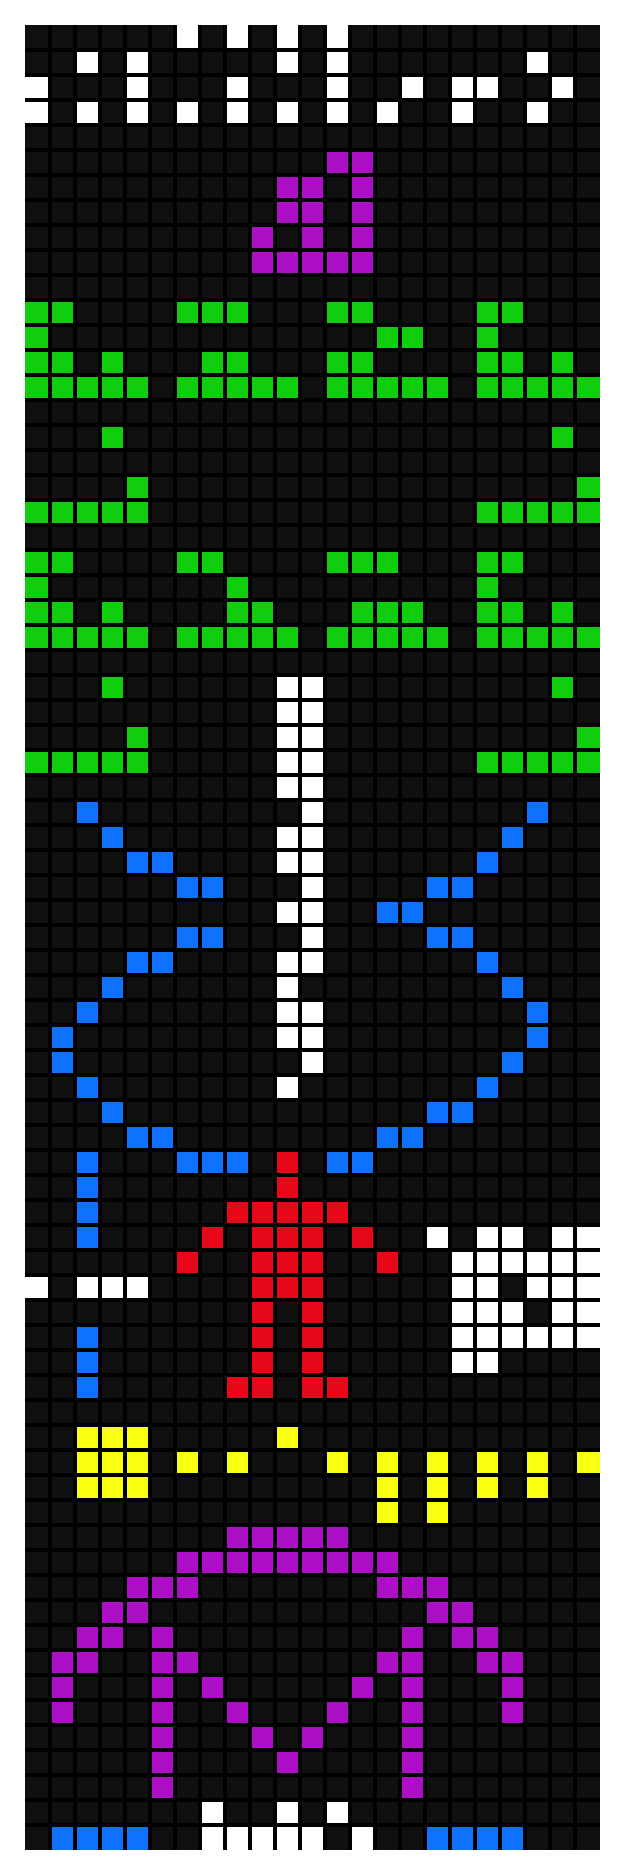
\includegraphics[height=9.1in]{Arecibo_message.pdf}
  };

  \node[anchor=east,inner sep=16pt,font=\bfseries] at (cover page.east) {
    \begin{minipage}[t]{3in}{
     \color{white}
        Jakob Vo\ss

	\vspace{1em}

        \resizebox{2.9in}{!}{\begin{tabular}{@{}l@{}}
        Describing\\Data Patterns
        \end{tabular}}

	\vspace{1em}

	A general deconstruction\\
	of metadata standards

        \vspace{3.9in}
    }\end{minipage}
};
\end{tikzpicture}

% back cover
\begin{tikzpicture}[remember picture,overlay]
\node[yshift=-3em,text width=5.5in,text justified,
  anchor=north] at (back cover.north) {
\small
\input{../abstract.txt}
};

% barcode
%\node[anchor=south east,
%    fill=white,minimum width=2in,minimum height=1.2in,
%    xshift=-2\bleedmargin,yshift=2\bleedmargin] 
%at (back cover.south east) {
%\begin{pspicture}(2in,1.2in)
%\psbarcode[scalex=0.8,scaley=0.8]{978-3-86541-114}{includetext}{isbn}
%\end{pspicture}
%};
\end{tikzpicture}



\end{document}
